\section{轴主视图生成}\label{sec:zhoushitu}
\begin{procedure}
\item 保存轴三维模型的副本

将轴的三维模型另存为“轴视图布局.dwg”。之所以要保存副本,一是为了防止视图布局操作对模型文件的影响,二是可以多次使用。

\yaodian{进行三维模型的视图布局操作之前,保存副本是一个良好的习惯。}

\item 将模型空间切换图纸空间

AutoCAD默认开始工作的空间是模型空间。模型空间是一个无限的三维绘图区域,可以用于制作1:1的二维图或三维模型。AutoCAD的图纸空间则主要用于图形输出准备。在图形空间中可以设置带有标题栏和注释的不同布局。在每个布局中,可以创建显示模型空间的不同视图的布局视口。在布局视口中,可以相对于图纸空间缩放模型空间视图。由此可见图纸空间可以实现形式多样的图形输出方式,模型空间更加灵活。

在AutoCAD中实现由模型空间切换为比较方便,用鼠标单击命令提示窗口上面的选项卡,使其由模型状态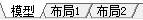
\includegraphics[scale=0.6]{moxinkongjian.png} 切换为布局状态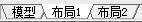
\includegraphics[scale=0.6]{bujukongjian.png} 即可。切换后,会出现图\ref{fig:morenbuju}所示的默认布局。

\begin{figure}[htbp]
\centering
\begin{floatrow}[2]
\ffigbox{\caption{默认布局}\label{fig:morenbuju}}{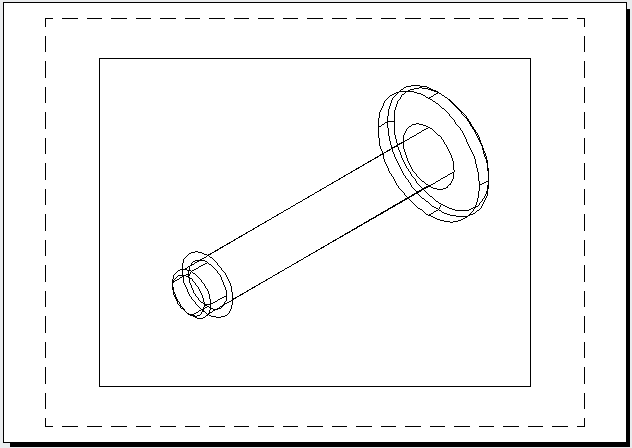
\includegraphics[scale=0.4]{morenbuju.png}}
\ffigbox{\caption{布局右键菜单}\label{fig:bujurightmeum}}{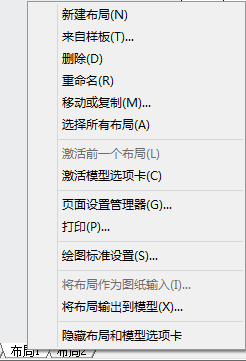
\includegraphics[scale=0.5]{bujurightmeum.png}}
\end{floatrow}
\end{figure}

\item 修改页面设置

通常默认布局的页面设置并不能够满足实际图纸输出的需求,因此需要修改布局的设置。AutoCAD启动页面设置管理器的方法有:
\begin{itemize}
\item 键盘输入 paggesetup\index{pagesetup,页面设置管理器}。
\item 【文件】$\rightarrow$【页面设置管理器】$\rightarrow$【并集】。
\item 在布局选项卡上右击鼠标,弹出图所示\ref{fig:bujurightmeum}菜单,然后选择【页面设置管理器】项。
\end{itemize}

\begin{lstlisting}
命令:pagesetup
\end{lstlisting}

页面设置管理器启动后,会弹出图\ref{fig:pagesetup}所示对话框。此时,单击修改按钮,弹出图\ref{fig:pagesetupdetail}所示的页面设置对话框。然后按照图\ref{fig:pagesetupdetail}的设置,将打印机绘图设备修改为“DWG TO PDF.pc3”,图纸尺寸设置为ISO A4(210.00x297.00毫米),其它参数保持不变。实际工作中应该打印机绘图设备设置为能够正常输出图形的真实打印机,才能够真正实现图形的打印输出。本书的设置是将AutoCAD的文件以PDF的形式输出,用以演示图形输出结果。设置完成后,单击确定退出页面设置对话框。

\begin{figure}[htbp]
\centering
\subfloat[]{\label{fig:pagesetup}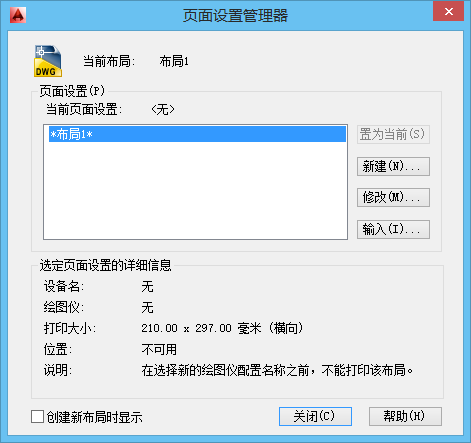
\includegraphics[scale=0.35]{pagesetup.png}}
\hspace{20pt}
\subfloat[]{\label{fig:pagesetupdetail}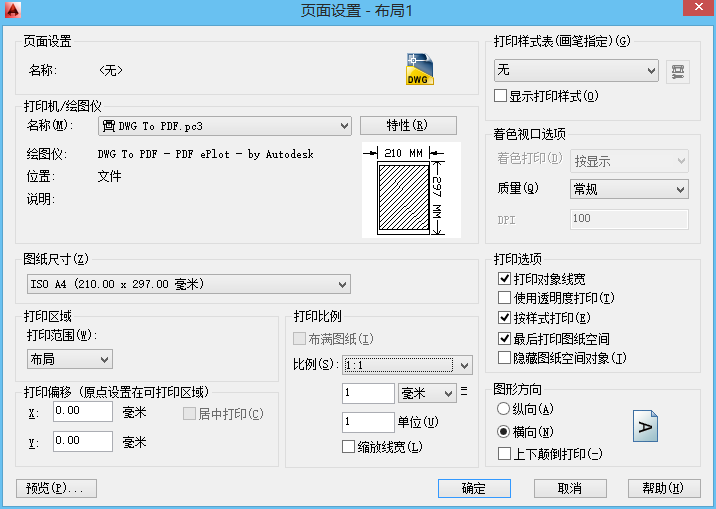
\includegraphics[scale=0.3]{pagesetupdetail.png}}
\caption{修改页面设置}
\end{figure}

\item 进入视口的模型空间

为了完成后续操作,我们需要进入图纸空间中视口的模型空间状态,通常完成操作有两种方式:
\begin{itemize}
\item 键盘输入MSPACE\index{mspace,视口模型空间}或MS。
\item 用鼠标双击图\ref{fig:selectshikou}中包含三维模型的矩形框的中间位置。
\end{itemize}

\begin{lstlisting}
命令:mspace
\end{lstlisting}

进入视口的模型空间后,视口的边框以粗实线的试标识,表示视口处于激活状态,其结果如图\ref{fig:selectshikouruslt}所示。
\begin{figure}[htbp]
\centering
\subfloat[]{\label{fig:selectshikou}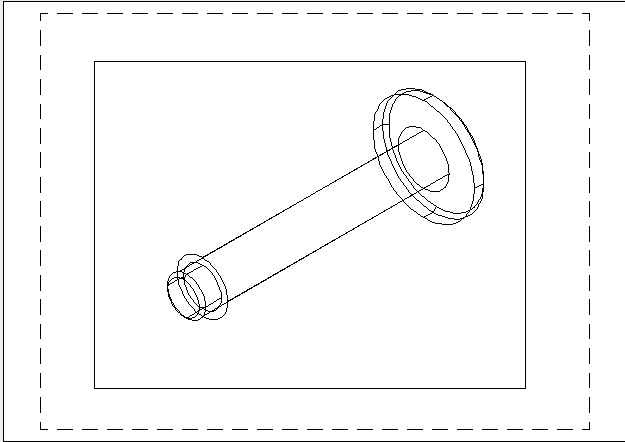
\includegraphics[scale=0.3]{selectshikou.png}}
\hspace{20pt}
\subfloat[]{\label{fig:selectshikouruslt}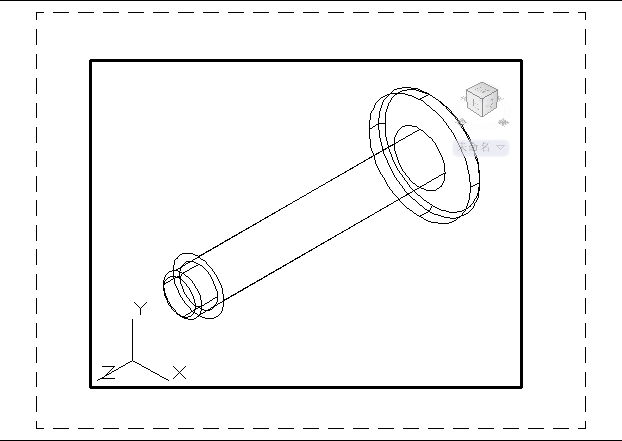
\includegraphics[scale=0.3]{selectshikouruslt.png}}
\caption{进入视口模型空间}
\end{figure}
\item 切换视图方向为前视图

为使生成的视图的方向与图\ref{fig:xiaolunzhou}所示的主视图方向一致,并且正投影图的方式进行显示,需要将视图方向切换换为前视图。

\begin{figure}[htbp]
\centering
\begin{floatrow}[2]
\ffigbox{\caption{视图切换结果}\label{fig:bujuforntview}}{
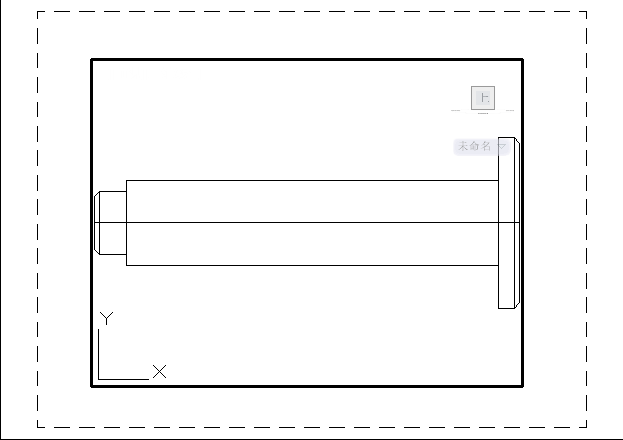
\includegraphics[scale=0.4]{bujuforntview.png}}
\ffigbox{\caption{工具栏设置}\label{fig:toolsset}}{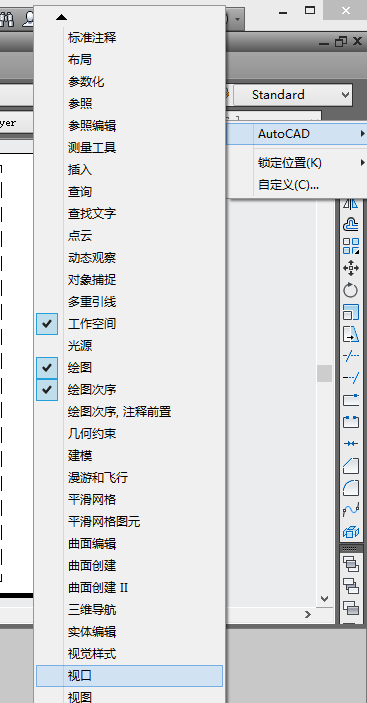
\includegraphics[scale=0.25]{toolsset.png}}
\end{floatrow}
\end{figure}
\begin{lstlisting}

命令: -VIEW
输入选项 [?/删除(D)/正交(O)/恢复(R)/保存(S)/设置(E)/窗口(W)]: front
\end{lstlisting}

切换完成后,其结果如图\ref{fig:bujuforntview}所示。
\item 设置视口显示比例
为使生成的视图以国家标准规定的比例显示,我们需要在视口比例文本框
\includegraphics[scale=0.5]{shikoutools.png}  中将比例设置为5:1
\includegraphics[scale=0.5]{shikoutools2.png}。

通常情况下,AutoCAD经典模式的视口工具栏默认是不显示的,需要在AutoCAD工具栏的空白处右击,弹出图\ref{fig:toolsset}所示的菜单,勾选视口,即可弹出视口工具栏
\includegraphics[scale=0.5]{shikoutools.png}。
\item 提取主视图

要从三维模型中提取主视图需要用AutoCAD中的轮廓命令,其调用方法有:
\begin{itemize}
\item 键盘输入SOLPROF\index{solprof,轮廓}。
\item 【绘图】$\rightarrow$【建模】$\rightarrow$【设置】$\rightarrow$【轮廓】。
\end{itemize}
\begin{lstlisting}
命令: solprof
选择对象: 找到 1 个
选择对象:
\end{lstlisting}
命令调用后,提示选择对象,此时按照图\ref{fig:lunkuoselect}的方式选择轴对象。选择完成后轴对象会以图\ref{fig:lunkuoselectresult}所示的虚线方式予以标识。
\begin{figure}[htbp]
\centering
\subfloat[]{\label{fig:lunkuoselect}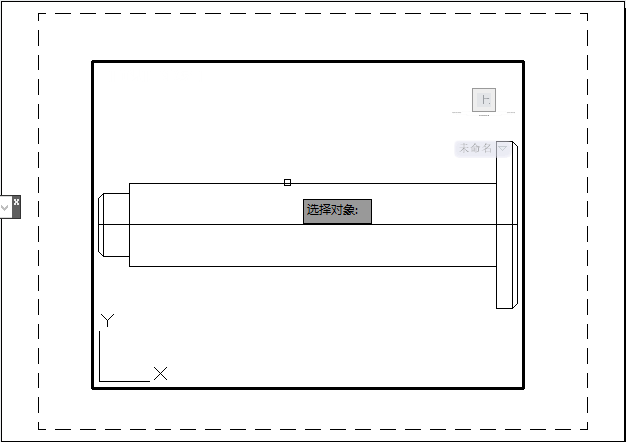
\includegraphics[scale=0.3]{lunkuoselect.png}}
\hspace{20pt}
\subfloat[]{\label{fig:lunkuoselectresult}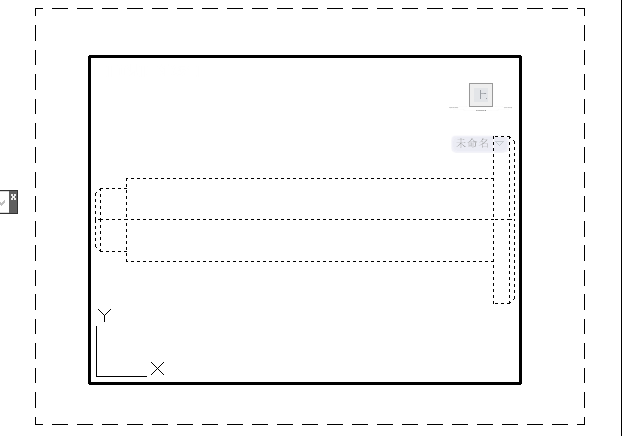
\includegraphics[scale=0.3]{lunkuoselectresult.png}}
\caption{轮廓操作}
\end{figure}

选择完成后,直接按空格键结束对象选择,此时提示是否在单独的层中显示隐藏轮廓线,默认值是“是”,故直接按空格键确认。
\begin{lstlisting}
是否在单独的图层中显示隐藏的轮廓线?[是(Y)/否(N)] <是>:
\end{lstlisting}
接下来提示是否将轮廓线投影到平面,其默认值是“是”,也直接以空格键确认。
\begin{lstlisting}
是否将轮廓线投影到平面?[是(Y)/否(N)] <是>:
\end{lstlisting}
最后提示是否删除相切的边,根据我们的制图标准相切边是不用表示的,故选择删除相切边。
\begin{lstlisting}
是否删除相切的边? [是(Y)/否(N)] <是>:
\end{lstlisting}

%\begin{lstlisting}
%_.VPLAYER 输入选项 [?/颜色(C)/线型(L)/线宽(LW)/透明度(TR)/冻结(F)/解冻(T)/重置(R)/新建冻结(N)/视口默认可见性(V)]: _N
%输入在所有视口中都冻结的新图层的名称: PV-28C 输入选项 [?/颜色(C)/线型(L)/线宽(LW)/透明度(TR)/冻结(F)/解冻(T)/重置(R)/新建冻结(N)/视口默认可见性(V)]: _T
%输入要解冻的图层名: PV-28C
%指定视口 [全部(A)/选择(S)/当前(C)/当前以外(X)] <当前>: 输入选项 [?/颜色(C)/线型(L)/线宽(LW)/透明度(TR)/冻结(F)/解冻(T)/重置(R)/新建冻结(N)/视口默认可见性(V)]:
%命令: _.VPLAYER 输入选项 [?/颜色(C)/线型(L)/线宽(LW)/透明度(TR)/冻结(F)/解冻(T)/重置(R)/新建冻结(N)/视口默认可见性(V)]: _NEW
%输入在所有视口中都冻结的新图层的名称: PH-28C 输入选项 [?/颜色(C)/线型(L)/线宽(LW)/透明度(TR)/冻结(F)/解冻(T)/重置(R)/新建冻结(N)/视口默认可见性(V)]: _T
%输入要解冻的图层名: PH-28C
%指定视口 [全部(A)/选择(S)/当前(C)/当前以外(X)] <当前>: 输入选项 [?/颜色(C)/线型(L)/线宽(LW)/透明度(TR)/冻结(F)/解冻(T)/重置(R)/新建冻结(N)/视口默认可见性(V)]:
%\end{lstlisting}

\item 修改图层设置

经过前面的操作,已经完成了轴主视图的制作,但由于生成的视图与实体都被显示出来了,因而结果与图\ref{fig:xiaolunzhou}的结果存在着一些差异。要实现只显示与视图相关的内容,就需要修改AutoCAD的图层属性。 所谓图层就是将属性相同的对象绘制在一张类似于透明的纸上,将不同属性的对象绘制在不同的透明纸上,以实现图形对象的分类管理,最后将所有的透明纸叠加在一起就构成了整个图形。修改【图层】设置的方法有:
\begin{itemize}
\item 键盘输入LAYER\index{layer,图层}或LA。
\item 【格式】$\rightarrow$【图层】。
\item 【图层工具栏】 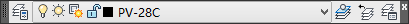
\includegraphics[scale=0.5]{layertoolsbar.png} $\triangleright$【图层】图标
\includegraphics[scale=0.6]{layertool.png}。
\end{itemize}
\begin{lstlisting}
命令:layer
\end{lstlisting}
图层命令调用后会弹出图\ref{fig:layerdialog}所示的图层对话框。整个图层对话框分为三个部分,分别是工具区、过滤器和图层列表。首先,在图层列表中选中以PV开头的图层,并单击
\includegraphics[scale=0.6]{setcurrentlayer.png}图标,将其设置为当前图层。然后单击该图层中线宽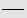
\includegraphics[scale=0.6]{linewidthselect.png} 图标,弹出图\ref{fig:linewidthset}对话框,选中0.50mm的线宽,点击确定,即可完成图层线宽的设置。最后点击0图层的
\includegraphics[scale=0.6]{layeronoffset.png}图标,使之切换为
\includegraphics[scale=0.6]{layeroffstatus.png}状态,实现对0图层的关闭。最终的图层设置结果如图所示

\begin{figure}[htbp]
\centering
\begin{floatrow}[2]
\ffigbox{\caption{图层对话框}\label{fig:layerdialog}}{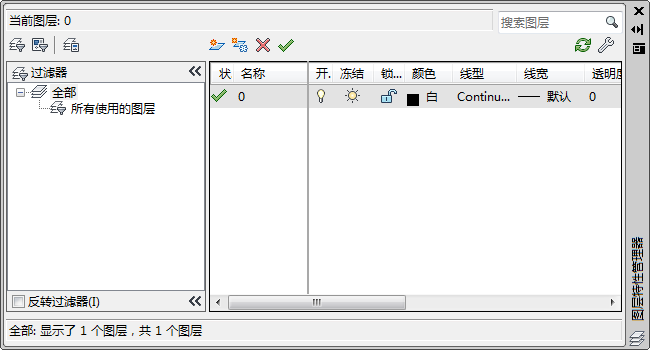
\includegraphics[scale=0.4]{layerdialog.png}}
\ffigbox{\caption{线宽设置对话框}\label{fig:linewidthset}}{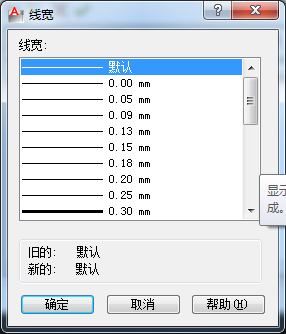
\includegraphics[scale=0.4]{linewidthset.png}}
\end{floatrow}
\end{figure}
\begin{figure}[htbp]
\centering
\begin{floatrow}[2]
\ffigbox{\caption{图层设置结果}\label{fig:layersetresult}}{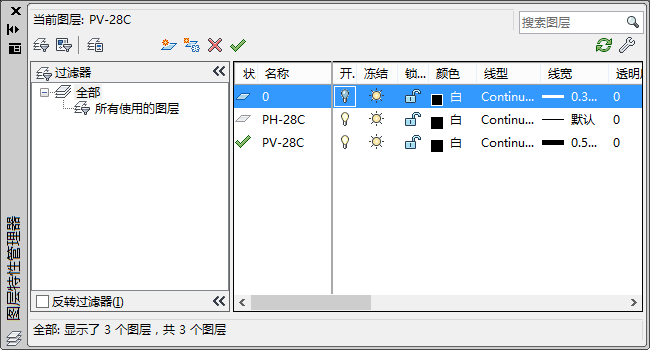
\includegraphics[scale=0.4]{layersetresult.png}}
\ffigbox{\caption{轴主视图}\label{fig:zhoushituresult}}{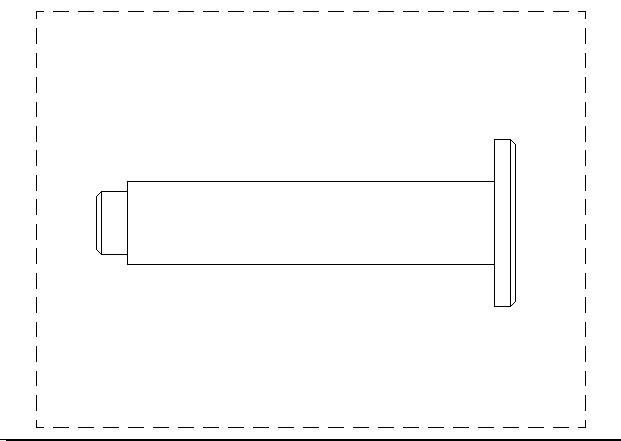
\includegraphics[scale=0.3]{zhoushituresult.png}}
\end{floatrow}
\end{figure}

\yaodian{处于关闭状态的图层,不会显示。但关闭图层的内容仍然存在。}

\item 返回图纸空间
至此,我们已经完成了轴主视图生成的所有操作,为了停止在视口模型空间中做缩放操作导致视图比例改变,因此需要返回图图纸空间。AutoCAD中返回图纸空间的方法有:
\begin{itemize}
\item 键盘输入 PSPACE\index{pspace,图纸空间}或PS。
\item 用鼠标双击视口以外的空白区域
\end{itemize}
\begin{lstlisting}
命令:pspace
\end{lstlisting}
返回图纸空间后,其结果如图 所示。从图中,可知生成的轴主视图与图\ref{fig:xiaolunzhou}的主视图是一致的。

\end{procedure}

\endinput